% !TEX TS-program = pdflatexmk
\documentclass[12pt]{article}

% Layout.
\usepackage[top=1in, bottom=0.75in, left=1in, right=1in, headheight=1in, headsep=6pt]{geometry}

% Fonts.
\usepackage{mathptmx}
\usepackage[scaled=0.86]{helvet}
\renewcommand{\emph}[1]{\textsf{\textbf{#1}}}
\newcommand{\ans}[1][1in]{\rule{#1}{.5pt}}

\usepackage[parfill]{parskip}

% Misc packages.
\usepackage{amsmath,amssymb,latexsym}
\usepackage{graphicx,hyperref}
\usepackage{array}
\usepackage{xcolor}
\usepackage{multicol,tikz}
\usepackage{tabularx,colortbl,booktabs,xparse}
\usepackage{enumitem}

% Rotation: \rot[<angle>][<width>]{<stuff>}
\NewDocumentCommand{\rot}{O{45} O{1em} m}{\makebox[#2][l]{\rotatebox{#1}{#3}}}%

\usepackage{fancyhdr}
\pagestyle{fancy} 
\lhead{\large\sf\textbf{MATH F113X: Kruskals's \& Dijkstra's Algorithm v2}}
%\chead{\large\sf\textbf{lecture notes}}
%\rhead{\large\sf\textbf{Day 1}}

\begin{document}
%\begin{minipage}{.4\linewidth}
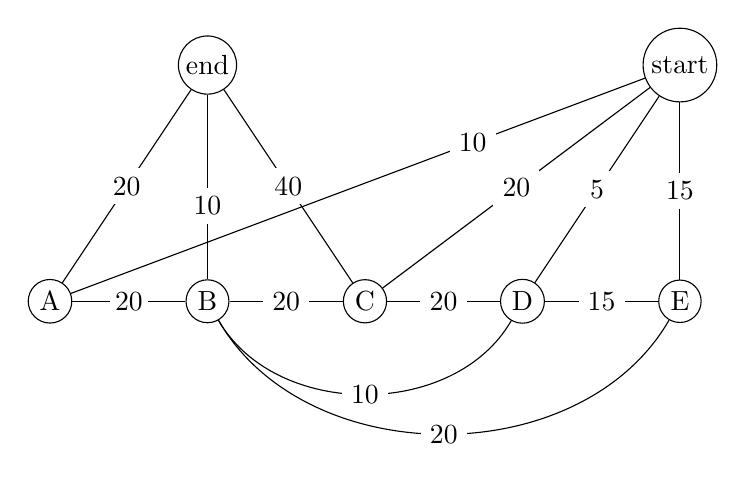
\begin{tikzpicture}[scale=1]
\node[draw,circle, inner sep=1.5pt](end) at (2,3){end};
\node[draw,circle, inner sep=2pt](a) at (0,0){A};
\node[draw,circle, inner sep=2pt](b) at (2,0){B};
\node[draw,circle, inner sep=2pt](c) at (4,0){C};
\node[draw,circle, inner sep=2pt](d) at (6,0){D};
\node[draw,circle, inner sep=2pt](e) at (8,0){E};
\node[draw,circle, inner sep=2pt](start) at (8,3){start};
\draw (end) -- (a) node [midway,fill = white]{20};
\draw (end) -- (b) node [midway,below,fill = white]{10};
\draw (end) -- (c) node [midway,fill = white]{40};
\draw (b) -- (c) node [midway,fill = white]{20};
\draw (a) -- (b) node [midway, inner sep = 2pt, fill = white]{20};
\draw (b) to[out=300, in=240] node[midway, fill = white] {20}(e);
\draw (b) to[out=300, in=240] node[midway, fill = white] {10}(d);
\draw (d) -- (e) node [midway,fill = white]{15};
\draw (c) -- (d) node [midway,fill = white]{20};
\draw (start) -- (e) node [midway,fill = white]{15};
\draw (start) -- (d) node [midway,fill = white]{5};
\draw (start) -- (c) node [midway,fill = white]{20};
\draw (start) -- (a) node [pos = .3,fill = white]{10};
\end{tikzpicture}
%\end{minipage}
%%%%%%%
% 
\vspace{0.5in}

 \begin{tabular}{c||c|c|c|c|c|c|c}
 & \textbf{end} & \textbf{A} & \textbf{B} & \textbf{C} & \textbf{D} & \textbf{E} & \textbf{start} \\ \hline \hline
\textbf{end}   &    & 20 & 10 & 40 &    &    &    \\ \hline
\textbf{A}     & 20 &    & 20 &    &    &    & 10 \\ \hline
\textbf{B}     & 10 & 20 &    & 20 &  10  & 20 &    \\ \hline
\textbf{C}     & 40 &    & 20 &    & 20 &    & 20 \\ \hline 
\textbf{D}     &    &    & 10   & 20 &    & 15 & 5  \\ \hline
\textbf{E}     &    &    & 20 &    & 15 &    & 15 \\ \hline
\textbf{start} &    & 10 &    & 20 & 5  & 15 &    \\ \hline
\end{tabular}
 \hspace{.5in}
 \begin{tikzpicture}[scale=1, baseline={(current bounding box.center)}]
\node[draw,circle, inner sep=1.5pt](end) at (2,3){end};
\node[draw,circle, inner sep=2pt](a) at (0,0){A};
\node[draw,circle, inner sep=2pt](b) at (2,0){B};
\node[draw,circle, inner sep=2pt](c) at (4,0){C};
\node[draw,circle, inner sep=2pt](d) at (6,0){D};
\node[draw,circle, inner sep=2pt](e) at (8,0){E};
\node[draw,circle, inner sep=2pt](start) at (6,-3){start};
\end{tikzpicture}

\vspace{0.5in}
%
%  \begin{minipage}[t]{.6\linewidth}
 \begin{tabular}{ |c | c |c| c|}
 \hline
 &&\textbf{tentative}&\\
 vertex & current/ & minimum& preceding\\ 
 &visited&\quad distance to $end$ \quad& vertex\\
 \hline
start&&& \\
\hline 
A&&& \\
\hline 
B&&& \\
\hline 
C&&& \\
\hline 
D&&& \\
\hline 
E&&& \\
\hline 
end&&& \\
\hline 
 \end{tabular}

 % \end{minipage}
  \hfill
 
\newpage

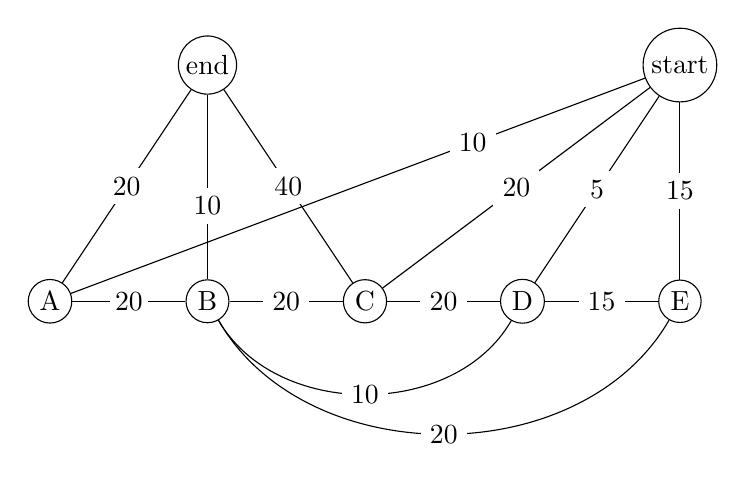
\begin{tikzpicture}[scale=1]
\node[draw,circle, inner sep=1.5pt](end) at (2,3){end};
\node[draw,circle, inner sep=2pt](a) at (0,0){A};
\node[draw,circle, inner sep=2pt](b) at (2,0){B};
\node[draw,circle, inner sep=2pt](c) at (4,0){C};
\node[draw,circle, inner sep=2pt](d) at (6,0){D};
\node[draw,circle, inner sep=2pt](e) at (8,0){E};
\node[draw,circle, inner sep=2pt](start) at (8,3){start};
\draw (end) -- (a) node [midway,fill = white]{20};
\draw (end) -- (b) node [midway,below,fill = white]{10};
\draw (end) -- (c) node [midway,fill = white]{40};
\draw (b) -- (c) node [midway,fill = white]{20};
\draw (a) -- (b) node [midway, inner sep = 2pt, fill = white]{20};
\draw (b) to[out=300, in=240] node[midway, fill = white] {20}(e);
\draw (b) to[out=300, in=240] node[midway, fill = white] {10}(d);
\draw (d) -- (e) node [midway,fill = white]{15};
\draw (c) -- (d) node [midway,fill = white]{20};
\draw (start) -- (e) node [midway,fill = white]{15};
\draw (start) -- (d) node [midway,fill = white]{5};
\draw (start) -- (c) node [midway,fill = white]{20};
\draw (start) -- (a) node [pos = .3,fill = white]{10};
\end{tikzpicture}


\begin{tabular}{c|c|c}
\textbf{Used?} & \textbf{Edge} & \textbf{Weight} \\ \hline
 & D--start & 5 \\
& A--start & 10 \\
& BD & 10 \\
 & B--end & 10 \\
 & DE & 15 \\
 & E--start & 15 \\
 & AB & 20 \\
 & A--end & 20 \\
  & BC & 20 \\
 
 & BE & 20 \\

 & CD & 20 \\
 
 & C--start & 20 \\
 & C--end & 40 \\
\end{tabular}
\hfill
\begin{tikzpicture}[scale=1]
\node[draw,circle, inner sep=1.5pt](end) at (2,3){end};
\node[draw,circle, inner sep=2pt](a) at (0,0){A};
\node[draw,circle, inner sep=2pt](b) at (2,0){B};
\node[draw,circle, inner sep=2pt](c) at (4,0){C};
\node[draw,circle, inner sep=2pt](d) at (6,0){D};
\node[draw,circle, inner sep=2pt](e) at (8,0){E};
\node[draw,circle, inner sep=2pt](start) at (6,-3){start};
\end{tikzpicture}
\end{document}